\documentclass[10pt,twocolumn,a4paper]{article}


% Use Times-like font for pdfLaTeX
\usepackage{mathptmx}

% Set up page geometry
\usepackage[a4paper, margin=1in]{geometry}
\usepackage[utf8]{inputenc}
\usepackage[T1]{fontenc}
\usepackage[german]{babel} % Use 'english' for English text
\usepackage{amsmath}
\usepackage{graphicx}
\usepackage{geometry}
\usepackage{booktabs} % For professional tables
\usepackage{hyperref}
\usepackage{parskip} % Space between paragraphs
\usepackage[backend=biber]{biblatex}
\addbibresource{references.bib} % BibTeX file for references

% Header and footer
\usepackage{fancyhdr}
\pagestyle{fancy}
\fancyhead[L]{Spektroskopie}
\fancyhead[C]{Digitale Holographische Spektroskopie}
\fancyhead[R]{Lorenz Saalmann}
\fancyfoot[C]{\thepage}

\begin{document}

\setlength{\parindent}{0pt}

% Document starts here

\begin{titlepage}
    \centering
    \begin{figure}
        \centering
        
\includegraphics[width=0.3\textwidth]{images/jlu_logo.jpeg}
    \end{figure}
    \vspace*{2cm}
    \text{Ausarbeitung} \\
    \Large{Digitale Holographische Spektroskopie} \\
    \vspace{2cm}
    \normalsize
    \today \\
    \normalsize{Lorenz Saalmann (8104072)} \\
    \vfill
    \normalsize{{Spektroskopie, SS 25}} \\
    \small{PD Dr. Arash Rahimi-Iman, Dipl.-Ing.} \\
\end{titlepage}

\newpage

\section{Einführung}
\vspace{-0.3cm}
\hspace{.0cm}\fontsize{9}{0}{\bf{KI-unterstützt von GPT-3.5 \cite{AI}}}
\vspace{0.4cm}
\\
\small
Spektroskopie befasst sich mit der Wechselwirkung von Licht und Materie. Im Fokus steht dabei die Abhängigkeit der Lichtintensität von Wellenlänge oder Frequenz. Damit lassen sich Phänomene wie Absorption, Emission und Streuung untersuchen. Da die beschriebene Wechselwirkung so grundlegend ist, findet die Spektroskopie in sehr vielen Bereichen Anwendung, wie zum Beispiel in der Chemie, Physik, Astronomie und Biologie. Sie dient der Materialanalyse, Zusammensetzungsbestimmung und der Untersuchung von physikalischen Eigenschaften von Stoffen. Konventionelle spektroskopische Verfahren basieren meist auf Intensitätsmessungen und liefern dadurch indirekte Informationen über Struktur oder Zusammensetzung eines Objekts. Insbesondere die Phaseninformation -- und damit quantitative Aussagen zur optischen Weglänge oder Topographie -- bleiben dabei unzugänglich.

Im Gegensatz dazu ermöglicht Holographie eine vollständige Erfassung des komplexen Lichtfeldes (Amplitude und Phase), wodurch eine hochauflösende dreidimensionale Rekonstruktion von Objekten möglich wird. Digitale Holographie überträgt dieses Prinzip in den digitalen Bereich: Mit modernen Bildsensoren und numerischen Rekonstruktionsverfahren lässt sich das holographisch aufgezeichnete Interferenzmuster analysieren. Kombiniert mit spektralen Messmethoden entsteht so die Digitale Holographische Spektroskopie (DHS). So können phasen-sensitive, räumliche und spektrale Informationen gleichzeitig erfasst werden, was eine tiefe Analyse des Lichtfeldes ermöglicht. Besonders in der Nanophotonik, der biomedizinischen Bildgebung und der Untersuchung optischer Materialien bietet DHS entscheidende Vorteile.

\section{Grundlagen der Holographie}
Ähnlich wie bei Photographie, ist das Ziel der Holographie, ein Objekt abzubilden. Der entscheidende Unterschied ist, dass dabei nicht nur die Intensität des Lichts an jedem Punkt auf einem Film erfasst, sondern auch dessen Phase. Dadurch bleibt die Tiefeninformation des Lichtfeldes erhalten und es ist möglich das Lichtfeld des Objekts sehr genau zu reproduzieren. Entdeckt wurde die Holographie von Dénes Gábor, einem ungarischen Ingenieur, 1947. Entscheidend für die Aufnahme dieser Informationen ist Interferenz. Eine monochromatische, kohärente Lichtquelle wird genutzt und in einen Referenzstrahl und einen Objektstrahl aufgeteilt. Bei einem Transmissionshologramm fällt die Referenz schräg auf den Film und interferiert mit dem Objektstrahl, nachdem dieser vom Objekt reflektiert wurde. So ist die Information über die Entfernung zum Objekt in dem Interferenzmuster in jedem Punkt erhalten, wobei die Auflösung des Films begrenzend wirkt. Um ein physisches Transmissionshologramm darzustellen, wird das auf Film aufgenommene Interferenzmuster nur mit dem Referenzstrahl beleuchtet. Das Muster wirkt dann als Beugungsgitter und das hinter dem Gitter resultierende Lichtfeld enthält das des Objektstrahls \cite{Gabor}.

Beim Betrachten ist ein virtuelles Bild des Objekts sichtbar, was beidäugig den vollständigen dreidimensionalen Eindruck des Objekts gibt. Teilt man den Film, kann durch beide Teile das gesamte Bild unter dem richtigen Winkel gesehen werden. Das gibt einen Hinweis darauf, dass Hologramme eine große Menge an Informationen speichern können.

Die Intensität des überlagerten Feldes kann als das Betragsquadrat der komplexen Wellen $R$ und $O$ beschrieben werden \cite{DHM}:
\begin{equation}
    |R + O|^2 = |R|^2 + |O|^2 + R^* O + R O^*.
\end{equation}
So kann das Interferenzmuster auf dem Film beschrieben werden. Wird dieses nun zur Rekonstruktion mit der Referenz $R$ beleuchtet, ergibt sich:
\begin{equation}
    R(|R|^2 + |O|^2 + R^* O + R O^*) = R(|R|^2 + |O|^2) + |R|^2O + |R|^2O^*.
\end{equation}
Hier kann man erkennen, dass die Objektwelle $O$ und ihr konjugiert komplexes $O^*$ um $|R|^2$ skaliert, sowie eine Referenzwelle.

\begin{figure}
    \centering
    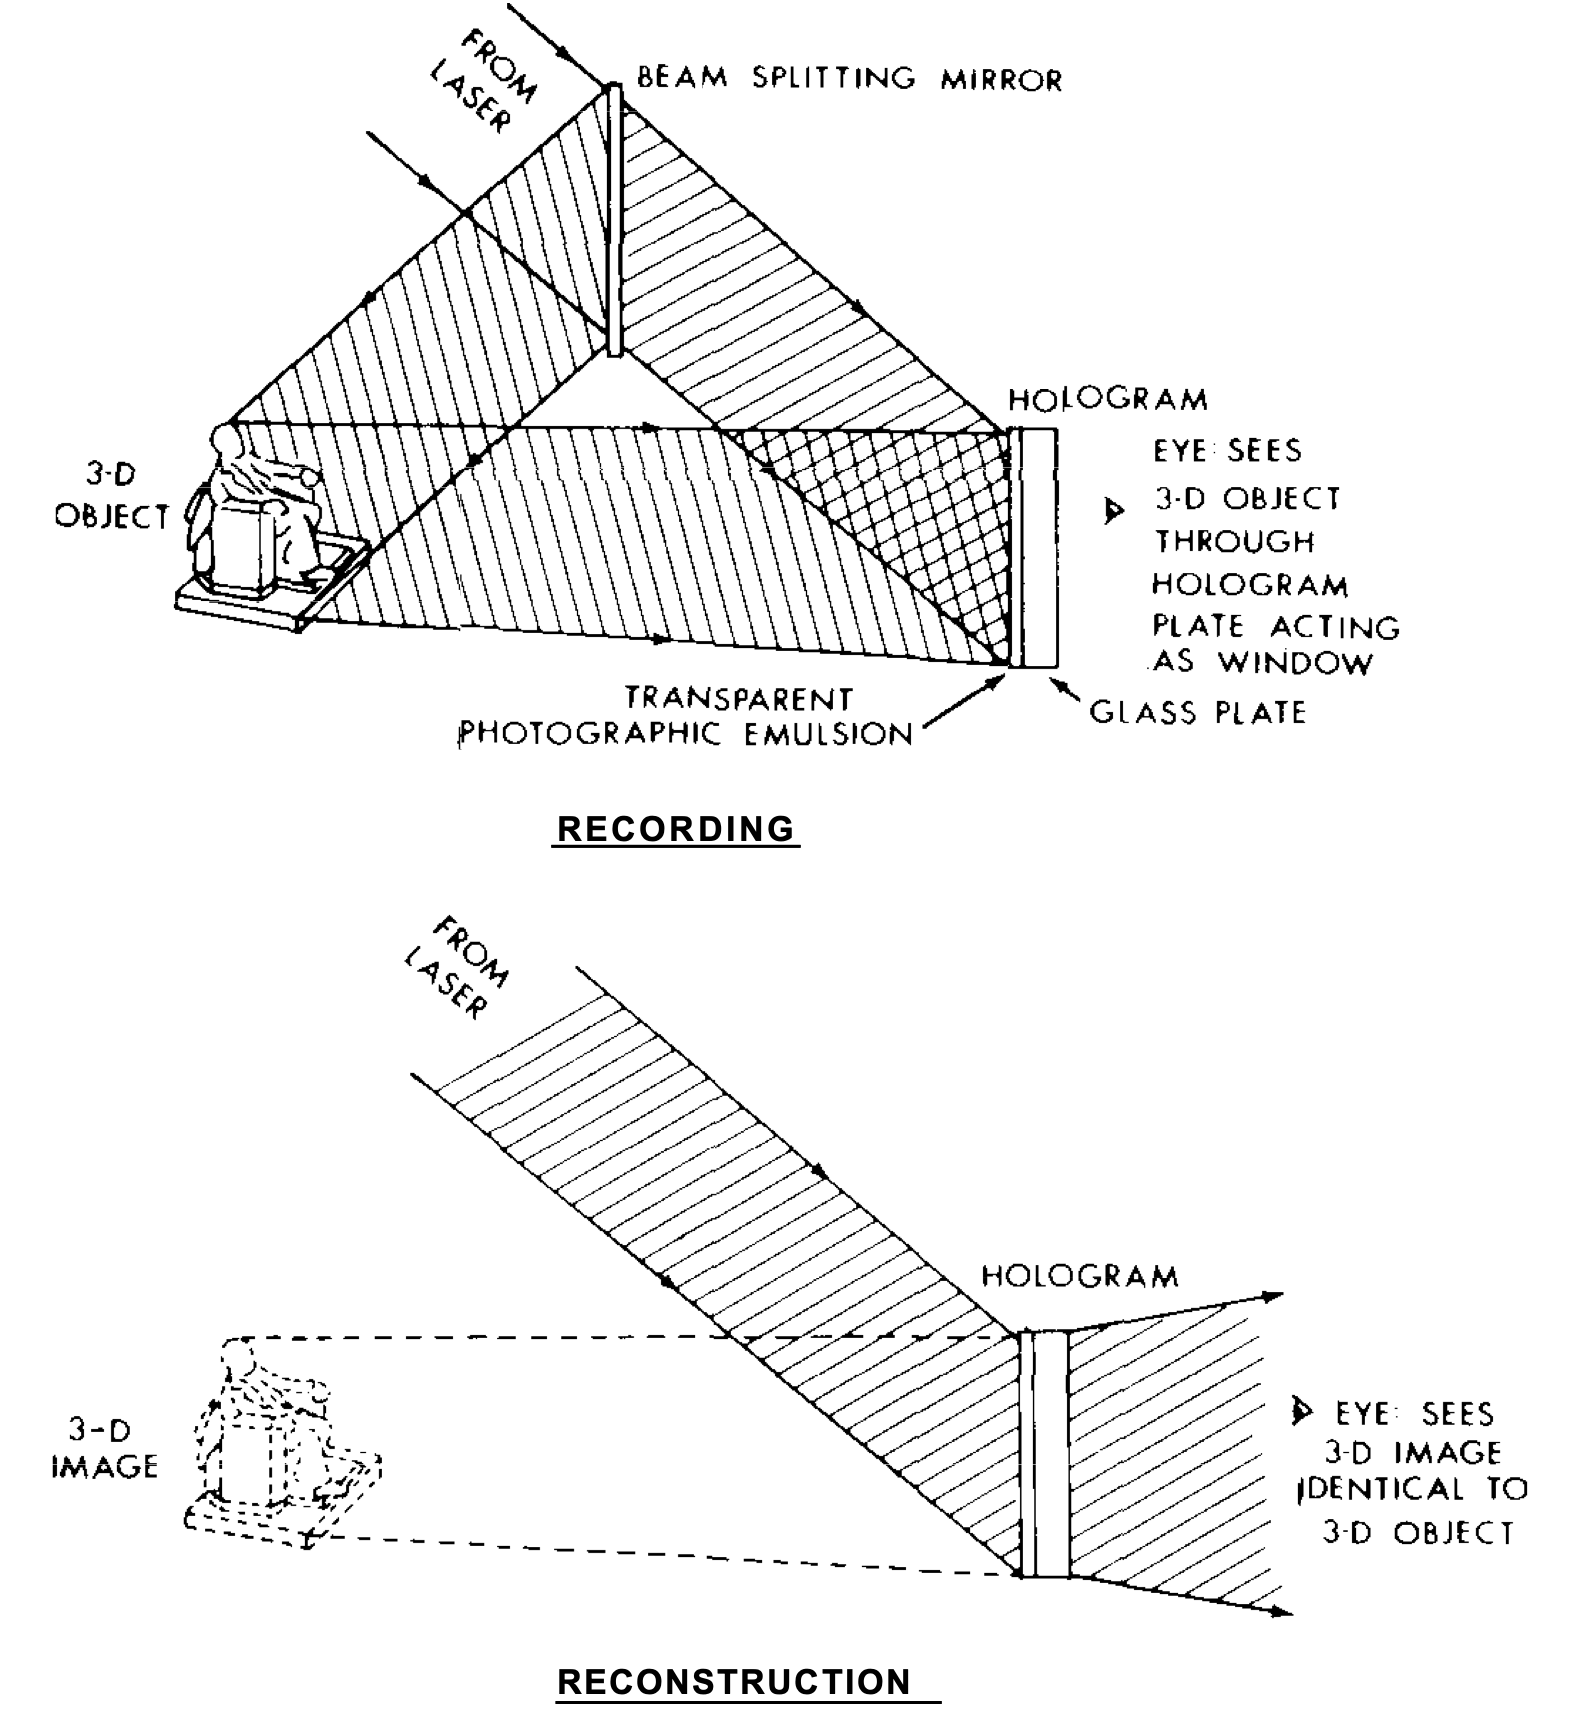
\includegraphics[width=0.5\textwidth]{images/holography.png}
    \caption{Prinzip der Holographie: Interferenz zwischen Referenz- und Objektstrahl bei einem Transmissionshologramm aus \cite{Gabor}.}
    \label{fig:holography}
\end{figure}

\section{Digitale Holographie}
Moderne Technik hat die Möglichkeiten in der Holographie seit den 50er-Jahren stark erweitert. Digitale Holographie nutzt CCD- oder CMOS-Sensoren, um die Interferenzmuster aufzuzeichnen, was die Auflösung und Empfindlichkeit stark erhöht. Anstatt einer Belichtung des Films mit der Referenzwelle kann aus dem Interferenzmuster numerisch der vom Objekt reflektierte Anteil des Lichtfeldes rekonstruiert werden. Andersherum kann auch das von einem beliebigem simulierten Objekt ausgehende Interferenzmuster iterativ bestimmt werden, sodass Hologramme virtuelle Objekte abbilden können. Aufgrund der hohen Auflösung des aufgenommenen Musters kann das Lichtfeld sehr genau rekonstruiert werden. Dabei können sehr feine Details und Strukturen von Oberflächen, sowie deren Wechselwirkung mit Licht präzise erfasst werden. Außerdem ist es möglich durch eine Überlagerung eines Hologramms mit dem abgebildeten Objekt mikroskopische Verformungen festzustellen, die bei mechanischem oder thermischem Stress auftreten. Die digitale Holographie findet daher Anwendung in vielen Bereichen, wie der Materialwissenschaft, Datenspeicherung, Mikroskopie und Spektroskopie.

Um das komplexe Wellenfeld hinter dem Interferenzmuster zu rekonstruieren, muss Licht in allen Punkten nach dem Huygensschen-Prinzip als sphärische Elementarwellen propagiert werden. Mathematisch wird dies durch das Rayleigh-Sommerfeld-Integral beschrieben, welches die Wellengleichung im Raum exakt löst. Während eine direkte Lösung im Ortsraum numerisch nicht effizient ist, kann eine zweidimensionale Fourier-Transformation genutzt werden, um das Interferenzmuster in den Frequenzbereich zu transformieren und es spektral darzustellen. Dort kann die Ausbreitung über eine Multiplikation mit einer Transferfunktion erfolgen, die die Phasenentwicklung der Welle über die Distanz beschreibt. Dafür wird häufig die Fresnel-Approximation verwendet, die unter kleinen Winkelabweichungen eine gute Näherung liefert. Sie ist gegeben durch:
\begin{equation}
    H_{\text{Fresnel}}(f_x, f_y) = \exp\left(-i \pi \lambda z \left( f_x^2 + f_y^2 \right)\right),
    \label{eq:fesnel}
\end{equation}
wobei $f_x$ und $f_y$ die räumlichen Frequenzkomponenten sind, $\lambda$ die Wellenlänge des Lichts und $z$ die Ausbreitungsdistanz. Die quadratischen Frequenzkomponenten entsprechen den räumlichen Frequenzen im Bild, die durch die Fourier-Transformation des Interferenzmusters entstehen und beschreiben wie sehr das Licht gebeugt wird, bzw. wie viel seine Phase verschoben wird \cite{DH}. 

Nachdem das Lichtfeld im Frequenzbereich propagiert wurde, kann es durch eine inverse Fourier-Transformation zurück in den Ortsraum transformiert werden. Das Ergebnis ist ein rekonstruiertes komplexes Lichtfeld, das alle aufgenommenen Informationen über Amplitude und Phase enthält.

\section{Anwendung in der \\Spektroskopie}
Zusätzlich zu der räumlichen Auflösung von Objekten kann auch die Abhängigkeit des Lichtfeldes von der Wellenlänge untersucht werden. Für jede Wellenlänge ergibt sich ein anderes Interferenzmuster, welches einzeln betrachtet werden muss. Überlagern sich die Interferenzen verschiedener Wellenlängen, verliert das resultierende Muster an Informationen. Das kann umgangen werden: entweder sequentiell, durch die Aufnahme von Hologrammen bei verschiedenen Wellenlängen, oder parallel durch die Nutzung spektraler Zerlegung auf der Sensorseite. In beiden Fällen können Amplitude, Phase und Frequenz des Lichtfeldes erfasst werden, was eine vollständige Charakterisierung ermöglicht. Das resultierende Hologramm kann dann als eine Summe von Hologrammen für jede Wellenlänge $\lambda_k$ beschrieben werden:
\begin{equation}
    U(x, y) = \sum_k A(x, y, \lambda_k)\, e^{i \phi(x, y, \lambda_k)}\, \Delta\lambda,
\end{equation}
wobei $A$ die Amplitude, $\phi$ die Phase, $x$ und $y$ die Koordinaten im Bild und $\Delta\lambda$ das Abtastintervall ist.
Daraus resultiert die Möglichkeit dynamische oder chromatische Prozesse zu untersuchen, die Dispersion und spektral veränderte Absorption oder Emission von Licht beinhalten. Außerdem können so auch volle dreidimensionale Abbildungen mit Farbe rekonstruiert werden.

Das bietet einige Vorteile gegenüber konventioneller Spektroskopie, vor allem, weil die Informationen zu Struktur und Spektrum von derselben Aufnahme stammen. Jedem Punkt auf dem Objekt kann ein spektrale Frequenzspektrum zugeordnet werden, was genauere Analyse und Unterscheidung von Materialien innerhalb eines Hologramms ermöglicht. Die Phase ist außerdem sensitiv gegenüber des Brechungsindex des Materials, wobei auch Gradienten und Strukturen im Inneren von transparenten Objekten oder Schichten erfasst werden können \cite{industrial}. Das ist unter anderem für die Untersuchung von biologischen Proben von großer Bedeutung, da man die Struktur von Zellen oder organischen Materialien ohne färbende oder fluoreszierende Marker untersuchen kann. 

Auch in der Materialforschung kann DHS sehr genaue Analysen von Oberflächen und Kontaktflächen ermöglichen, da die Phaseninformation bei kleinen Wellenlängen eine hohe Empfindlichkeit gegenüber kleinster Veränderungen bietet. Sie wird daher auch oft für digitale Mikroskopie verwendet, wofür Gábor Holographie auch ursprünglich verwenden wollte \cite{DHM}. Ein weiterer Vorteil von Holografie-basierter Spektroskopie als Bilderfassung ist, dass keine Linse erforderlich ist, die das Objekt auflöst und durch ihre Abbildungsfehler die Qualität des Bildes einschränkt. Stattdessen kann bei der Rekonstruktion ein bestimmter Fokus über die Distanz $z$ in Formel \ref{eq:fesnel} eingestellt werden.

\section{Zusammenfassung}
\vspace{-0.3cm}
\hspace{.0cm}\fontsize{9}{0}{\bf{KI-generiert von GPT-3.5 \cite{AI}}}
\vspace{0.3cm}
\\
Digitale Holographische Spektroskopie kombiniert räumliche, spektrale und phasensensitive Bildgebung in einem einzigen Verfahren und ermöglicht so eine außergewöhnlich vollständige Erfassung des Lichtfeldes. Diese Informationsdichte eröffnet neue Perspektiven für die Analyse komplexer Systeme und Materialien. Mit fortschreitender Sensor- und Rechentechnologie wird DHS zunehmend zu einem Schlüsselwerkzeug in der hochpräzisen optischen Messtechnik.

\AtNextBibliography{\small}
\printbibliography
\end{document}